\documentclass[tikz,border=5pt]{standalone}
\usepackage{amsmath,amssymb}
\usetikzlibrary{arrows.meta}
\definecolor{curveblue}{HTML}{245C86}
\definecolor{accent}{HTML}{A65E2E}
\begin{document}
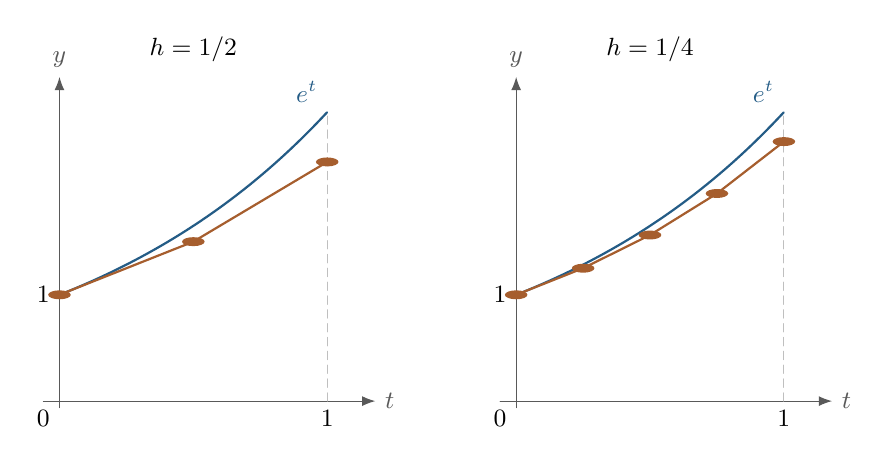
\begin{tikzpicture}[font=\small,>=Latex,line cap=round,line join=round]
\foreach \shift/\steps/\title in {0/2/{h=1/2},5.8/4/{h=1/4}} {
  \begin{scope}[shift={(\shift,0)},xscale=3.4,yscale=1.35]
    \draw[->,black!65] (-.06,0)--(1.18,0) node[right] {$t$};
    \draw[->,black!65] (0,-.06)--(0,3.05) node[above] {$y$};
    \draw[curveblue,thick,domain=0:1,samples=80] plot (\x,{exp(\x)});
    \node[curveblue,above left] at (1,{exp(1)}) {$e^t$};
    \node[above] at (.5,3.1) {$\title$};
    \node[below left] at (0,0) {$0$};
    \node[left] at (0,1) {$1$};
    \node[below] at (1,0) {$1$};
    \draw[densely dashed,black!25] (1,0)--(1,{exp(1)});
    \foreach \i in {0,...,\steps} {
      \pgfmathsetmacro{\tx}{\i/\steps}
      \pgfmathsetmacro{\yy}{pow(1+1/\steps,\i)}
      \fill[accent] (\tx,\yy) circle (1.2pt);
      \ifnum\i<\steps
        \pgfmathsetmacro{\nextx}{(\i+1)/\steps}
        \pgfmathsetmacro{\nexty}{pow(1+1/\steps,\i+1)}
        \draw[accent,thick] (\tx,\yy)--(\nextx,\nexty);
      \fi
    }
  \end{scope}
}
\end{tikzpicture}
\end{document}
